\subsubsection{Vorlesungen}
Wie in Abbildung \ref{fig:vorlesungen_reliability_score} zu sehen ist, hat bei den Vorlesungen unter Average Load kein Testdurchlauf einen Score über 50 von 100 Punkten erreicht.
Die k3s-Umgebung hat dabei wieder einen höheren Score als die Docker-Compose-Umgebung erhalten.
In den in Tabelle \ref{tab:vorlesungen_average_load_metrics} aufgeführten Messwerten ist besonders interessant, dass beide Umgebungen eine hohe Fehlerrate für eine Webanwendung aufweisen.
Dabei hat die k3s-Umgebung fast doppelt so viele Fehler wie die Docker-Compose-Umgebung.
Trotz der niedrigeren Fehlerrate hat die Anwendung in der Docker-Compose-Umgebung einen höheren CPU- und RAM-Verbrauch als die k3s-Umgebung.
\begin{table}[htbp]
\centering
\caption{Vergleich der Durchschnittswerte aller Test zur bestimmung der Zuverlässigkeit für das Vorlesungen-Szenario unter Average Load}
\label{tab:vorlesungen_average_load_metrics}

\begin{tabular}{lrr}
\toprule
\textbf{Metrik} & \textbf{Docker} & \textbf{K3s} \\
\midrule
Error Rate [\%]        & 2.38 & 4.65 \\
CPU Max [\%]           & 99.57 & 44.18 \\
Memory Max [\%]        & 74.66 & 23.58 \\
Node CPU Max [\%]      & 99.98 & 109.63 \\
Node Memory Max [\%]   & 81.25 & 81.02 \\
Restarts               & 0.00 & 0.00 \\
\bottomrule
\end{tabular}

\end{table}

\begin{figure}[htbp]
\centering
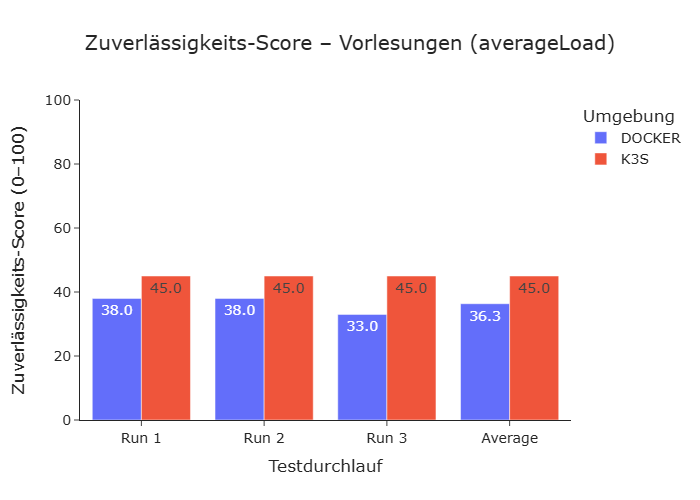
\includegraphics[width=0.8\textwidth]{bilder/tests/reliability_score_vorlesungen_averageLoad.png}
\caption{Reliability Score für das Vorlesungen-Szenario unter Average Load}
\label{fig:vorlesungen_reliability_score}
\end{figure}

Ein Vergleich der durchschnittlichen Zuverlässigkeitsscores jeder Testmethode in dem Szenario „Vorlesungen“, wie in Tabelle \ref{tab:scenario_score_matrix_vorlesungen} dargestellt, zeigt, dass die Docker-Compose-Umgebung in den meisten Testmethoden einen höheren Score erreichen konnte.
Nur beim „Average Load” konnte die „k3s”-Umgebung einen höheren Score als die „Docker Compose”-Umgebung erzielen. 
Bei „Smoke” haben beide Umgebungen wieder den gleichen Score erzielt.
Die Abstände zwischen den Umgebungen sind jeweils nicht allzu groß.

\begin{table}[htbp]
\centering
\caption{Durchschnittlicher Reliability Score pro Testtyp für das Szenario Vorlesungen}
\label{tab:scenario_score_matrix_vorlesungen}

\begin{tabular}{lccccc}
\toprule
\textbf{Environment} & \textbf{Smoke} & \textbf{Average Load} & \textbf{Stress} & \textbf{Spike} & \textbf{Breaking Point} \\
\midrule
Docker & 75.00 & 36.33 & 38.00 & 38.00 & 38.00 \\
K3s    & 75.00 & 45.00 & 31.67 & 25.00 & 25.00 \\
\bottomrule
\end{tabular}

\end{table}

\FloatBarrier